
%||||---------------
\begin{frame}[ctb!]
  \frametitle{Introduction : Purpose}
  Fuel cycle simulators are designed to answer policy-related questions
  regarding transitions from one equilibrium state to another.

  \vspace{0.2cm}

  \pause
  A simulator answers the following questions as a function of its 
  parameter space:
  \begin{itemize}
    \item how much material exists
    \item where does that material reside
    \item from/to where and when is material transported
    \item what kinds of facilities are needed
    \item when is each type of facility needed
  \end{itemize}
\end{frame}
%---------------||||

%||||---------------
\begin{frame}[ctb!]
  \frametitle{NESD Main Points}
  \begin{figure}[htbp!]
    \begin{center}
      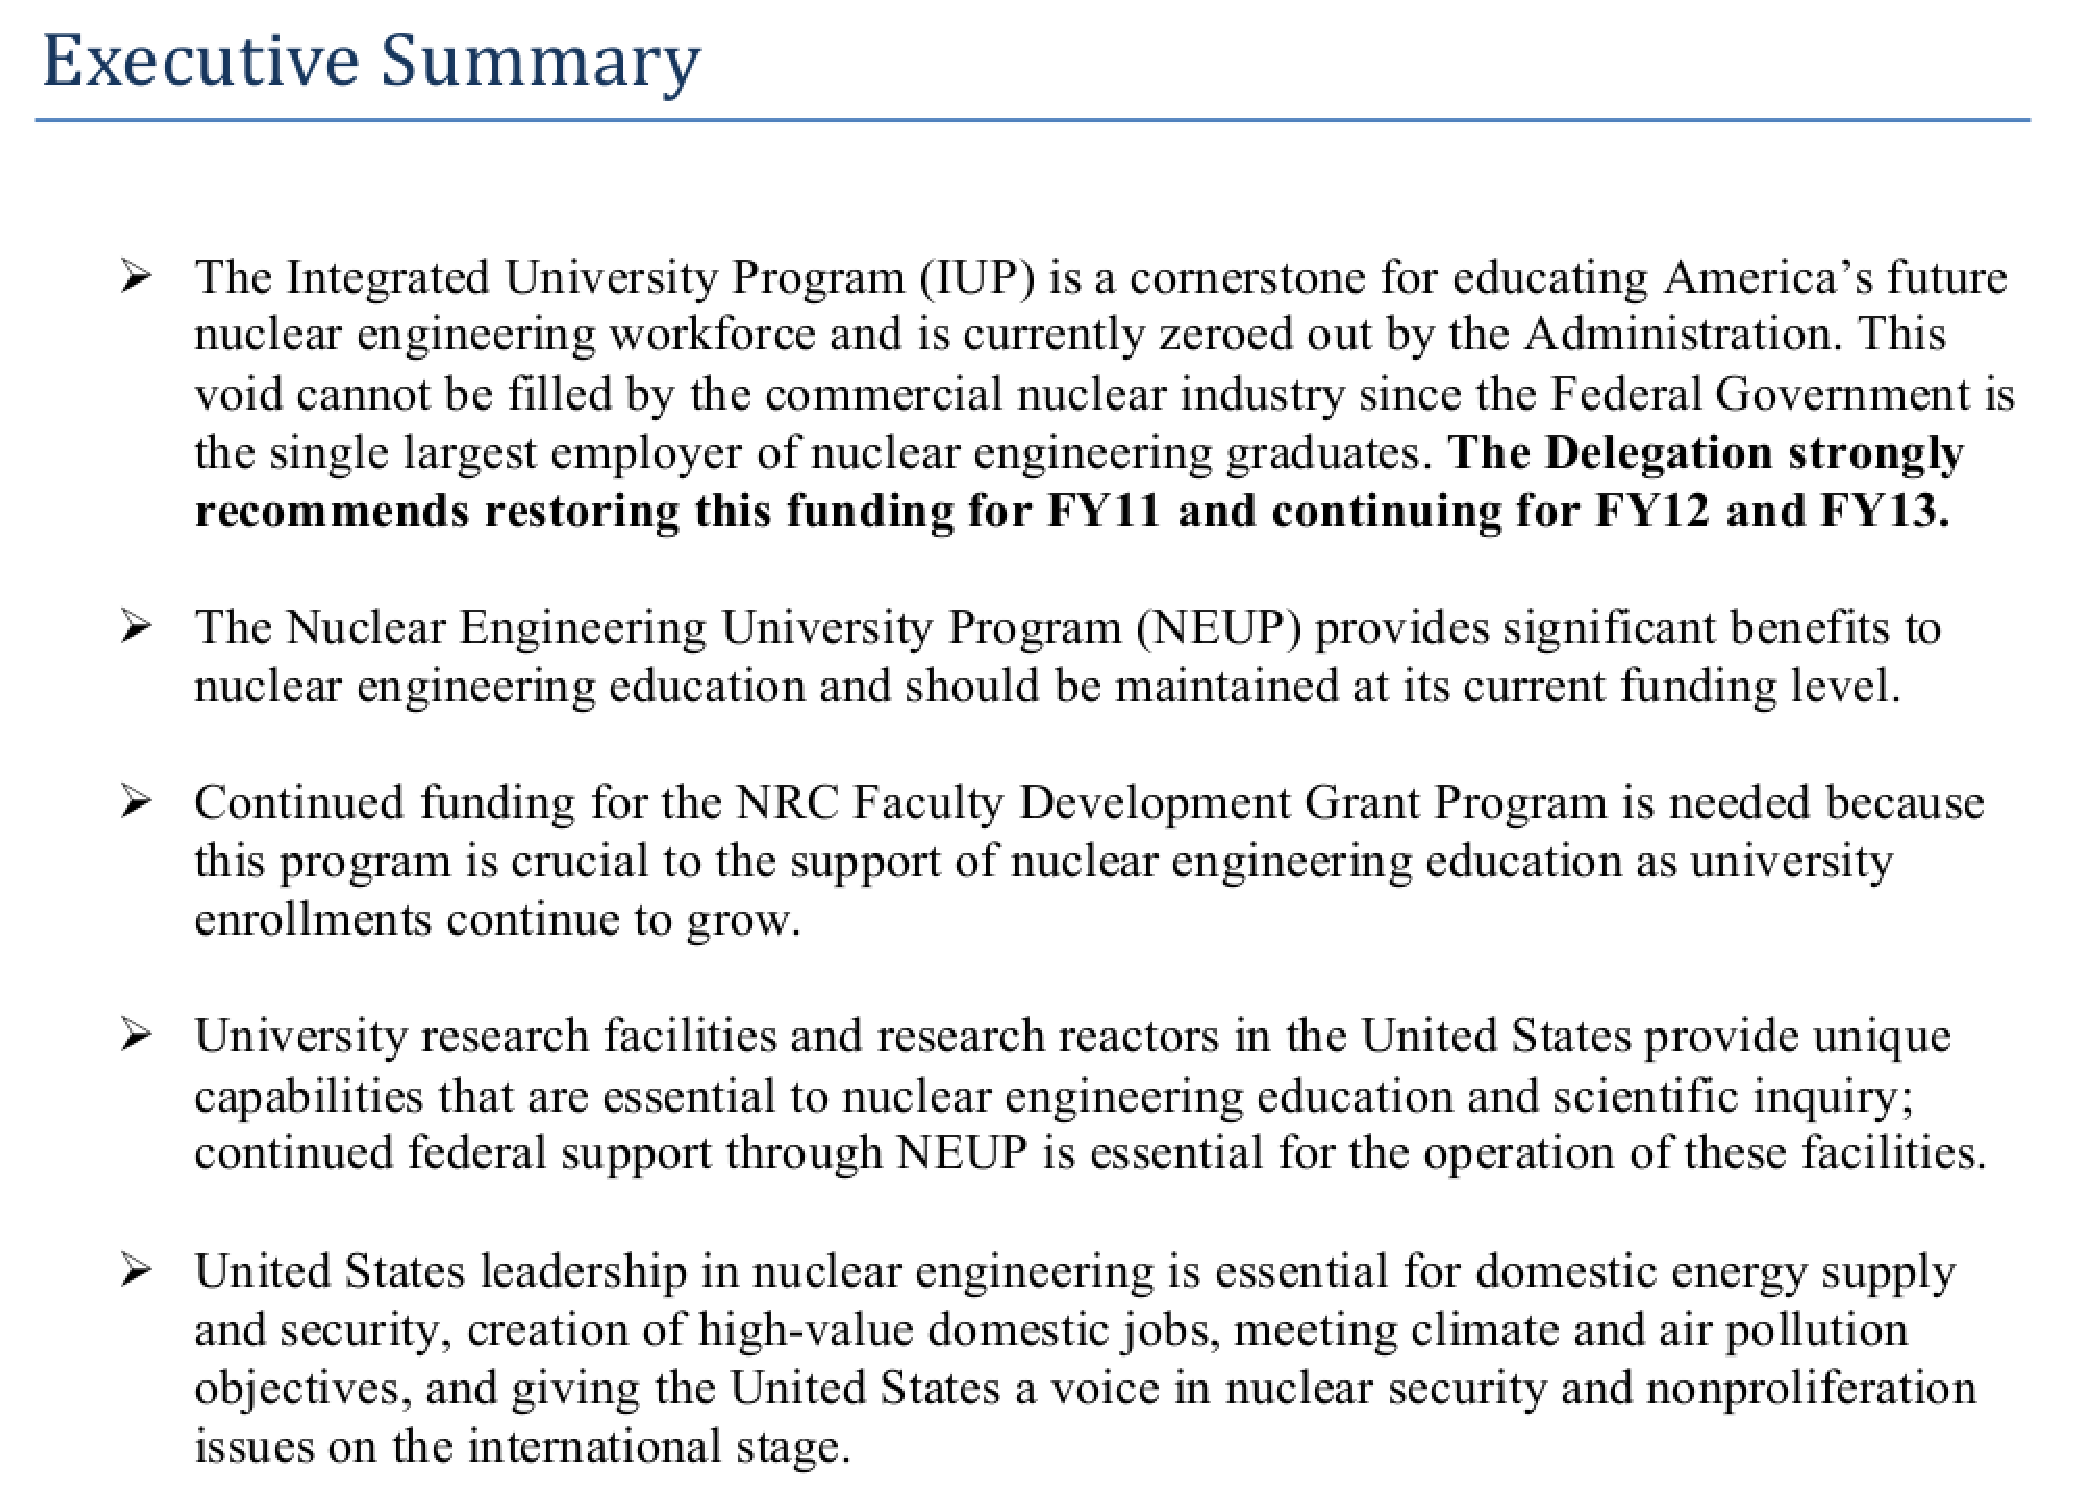
\includegraphics[height=5cm]{exec.eps}
    \caption{The NESD Executive Summary}
    \label{fig:exec}
    \end{center}
  \end{figure}
\end{frame}
%---------------||||
